\documentclass[10pt,twocolumn]{article}

\usepackage[letterpaper,margin=0.72in]{geometry}
\usepackage[T1]{fontenc}
\usepackage[utf8]{inputenc}
\usepackage{lmodern}
\usepackage{microtype}
\usepackage{amsmath,amssymb}
\usepackage{array}
\usepackage{booktabs}
\usepackage{graphicx}
\usepackage{listings}
\usepackage{tikz}
\usepackage{xcolor}
\usepackage{url}
\usetikzlibrary{arrows.meta,calc,positioning}

\raggedbottom
\emergencystretch=2em

\lstdefinelanguage{Jasmin}{
  morekeywords={fn,export,reg,mut,ptr,const,u32,u64,ui64,int,param,return,while,if,inline,require},
  sensitive=true,
  morecomment=[l]{//},
  morecomment=[s]{/*}{*/},
  morestring=[b]"
}

\lstset{
  language=Jasmin,
  basicstyle=\ttfamily\scriptsize,
  keywordstyle=\bfseries,
  columns=fullflexible,
  showspaces=false,
  showstringspaces=false,
  showtabs=false,
  % keepspaces=true,
  breaklines=true,
  frame=single,
  framerule=0.2pt,
  xleftmargin=2pt,
  xrightmargin=2pt,
  aboveskip=4pt,
  belowskip=4pt
}

\newcommand{\haetae}{HAETAE}
\newcommand{\jasmin}{Jasmin}
\newcommand{\ct}{constant-time}
\newcommand{\sct}{speculative constant-time}
\newcommand{\Zq}{\mathbb{Z}_q}
\newcolumntype{P}[1]{>{\raggedright\arraybackslash}p{#1}}
\colorlet{vizPublic}{blue!12!white}
\colorlet{vizSecret}{red!10!white}
\colorlet{vizSafety}{green!14!white}
\colorlet{vizSct}{violet!12!white}
\colorlet{vizCompiler}{orange!16!white}
\colorlet{vizLine}{black!62}
\tikzset{
  vizbox/.style={
    rectangle, rounded corners=2pt, draw=vizLine,
    minimum height=7.5mm, align=center,
    font=\scriptsize\sffamily, inner xsep=3pt, inner ysep=2pt
  },
  vizsmall/.style={
    rectangle, rounded corners=2pt, draw=vizLine,
    minimum height=6.2mm, align=center,
    font=\scriptsize\sffamily, inner xsep=2.5pt, inner ysep=1.8pt
  },
  viztag/.style={
    rectangle, rounded corners=1pt, draw=vizLine!80,
    align=center, font=\tiny\sffamily, inner xsep=2pt, inner ysep=1pt
  },
  vizarrow/.style={-Stealth, thick, draw=vizLine},
  vizdash/.style={-Stealth, thick, dashed, draw=vizLine},
  viznote/.style={font=\tiny\sffamily, align=center, text=black!72}
}

\title{\vspace{-0.8em}Safety and Constant-Time Verification of a Scalar \jasmin{} NTT for \haetae{}}
\author{Anonymous Submission}
\date{}

\begin{document}
\maketitle
\vspace{-1.1em}

\begin{abstract}
The number-theoretic transform (NTT) is a small but security-critical kernel in
lattice-based signature implementations.  Its low-level code must satisfy two
properties before functional correctness is meaningful as an implementation
claim: the program must be safe, so that every execution is defined, and it must
be constant time, so that branches and memory addresses do not depend on secret
polynomial coefficients.  This paper reports on the scalar \jasmin{}
implementation of the \haetae{} NTT, inverse NTT, and NTT-domain base
multiplication at this compiler-side layer.  The implementation is
stage-specialized so that the \jasmin{} safety checker can prove every
polynomial and twiddle-table access in bounds, and its exported wrappers carry
regular and speculative \ct{} annotations.  We describe how the current
\jasmin{} verification model specializes to this actual source code: typed
256-word polynomial pointers under caller validity preconditions, fixed public
loop schedules, public affine address expressions, secret coefficient
arithmetic, and entry fences emitted from \texttt{\#init\_msf()}.  The checked
artifact passes
\texttt{jasminc -checksafety}, \texttt{jasmin-ct}, and
\texttt{jasmin-ct --speculative}.  Together with the \jasmin{} compiler's
model-relative preservation discipline and byte-for-byte regeneration evidence
for \path{hpoly.s}, these checks give a source-to-assembly safety and
branch/address-timing argument for this generated scalar x86-64 code, not an
independent proof of arbitrary assembly or all physical side channels.
Functional correctness is a
separate layer: the companion EasyCrypt development currently proves the
forward and inverse NTT wrappers, while base multiplication is covered here only
by the safety and timing checks.
\end{abstract}

\section{Introduction}

Lattice-based signature schemes spend a large fraction of their running time in
polynomial arithmetic.  For \haetae{}~\cite{HAETAE2022}, the main transform is a
256-point NTT modulo \(q=64513\).  A fast implementation of this transform is
not just a mathematical program: it is a low-level in-place routine over machine
words, table pointers, loop counters, and ABI-visible entry points.  Two
classes of mistakes are particularly damaging.  First, an out-of-bounds table or
polynomial access can invalidate the execution model used by later proofs.
Second, a branch or memory address depending on a secret coefficient can leak
information even if the arithmetic result is correct.

This paper focuses on those two implementation properties for the scalar
\haetae{} NTT written in \jasmin{}~\cite{Jasmin2017,LastMile2020,JasminFramework2026}.
The source under
\path{jasmin/} implements three exported routines:
\path{poly_ntt_jazz}, \path{poly_invntt_jazz}, and
\path{poly_basemul_jazz}.  The code is compiled to x86-64 assembly
\path{hpoly.s}.  The same source is also suitable for extraction to EasyCrypt
for functional verification, but the present paper is about the compiler-side
guarantees that make the low-level execution well-defined and side-channel
disciplined.

The central claim is deliberately narrow and artifact-based.  The scalar
\jasmin{} implementation has been shaped so that the \jasmin{} toolchain proves
the following properties for the exported routines:
\begin{itemize}
  \item \textbf{Safety.}  All polynomial and twiddle-table accesses are within
        the 256-entry regions described by their types, assuming the caller
        supplies valid and aligned pointer arguments, and the primitive
        operations used by the program are well-defined in the \jasmin{}
        semantics.
  \item \textbf{Regular \ct{}.}  Branch conditions and memory addresses depend
        only on public loop counters, public stage constants, and public pointer
        bases, never on polynomial coefficients.
  \item \textbf{Speculative \ct{}.}  The exported wrappers establish a
        speculation boundary with \texttt{\#init\_msf()}, so transient pointer
        inputs become public address bases while pointed-to coefficients remain
        secret.
\end{itemize}

Table~\ref{tab:claim-boundaries} records the boundary of the claim up front.
This is useful because the paper sits between several verification layers: the
NTT mathematics, the \jasmin{} safety and timing checks, the compiler
preservation argument, and the separate EasyCrypt functional proof.  The paper
uses only the layers named in the evidence column.

\begin{table}[t]
\centering
\scriptsize
\setlength{\tabcolsep}{3pt}
\begin{tabular}{P{0.30\columnwidth}P{0.34\columnwidth}P{0.26\columnwidth}}
\toprule
Claim area & Evidence used here & Explicit non-claim \\
\midrule
Algorithmic target & HAETAE parameters, twiddle-table schedule, scalar
\jasmin{} source & New NTT algorithm or vectorized implementation \\
Safety & \texttt{jasminc -checksafety} logs and typed pointer preconditions &
Validity of arbitrary caller memory \\
Regular and speculative timing & \texttt{jasmin-ct}, \texttt{jasmin-ct
--speculative}, entry \texttt{lfence} shape & All microarchitectural leakage
channels \\
Functional correctness & Companion EasyCrypt forward/inverse NTT theorems &
Base-multiplication correctness or full signature security \\
\bottomrule
\end{tabular}
\caption{Claim boundaries for the submitted artifact.}
\label{tab:claim-boundaries}
\end{table}

The paper does not claim a new NTT algorithm, a vectorized implementation, or a
full signature-scheme proof.  Its contribution is the implementation-level
security argument for the scalar \jasmin{} kernels, grounded in the actual
source and the emitted assembly shape.  In particular, it records how a
helperized implementation exposes the exact obligations needed by the \jasmin{}
safety, regular \ct{}, and speculative \ct{} checkers.  This is a necessary
layer under any functional correctness theorem: a theorem about an extracted
model is only an implementation theorem if the compiled source is safe and
preserves the intended timing discipline.

The paper makes three concrete contributions.  First, it gives a code-level
description of the scalar HAETAE NTT, inverse NTT, and base-multiplication
kernels in the subset of \jasmin{} that matters to automatic safety and timing
checks.  Second, it separates the safety, regular \ct{}, SCT, compiler
preservation, and functional-correctness claims so that each statement has a
clear source of evidence.  Third, it packages reproducibility evidence for the
checked source and the generated scalar assembly.  The rest of the paper follows
that order: Section~2 describes the implementation target, Sections~3--7 explain
the verification models and arguments, Section~8 records the reproduced
evidence, and the final sections state the trust boundary and related work.

\begin{figure}[t]
\centering
\resizebox{\columnwidth}{!}{%
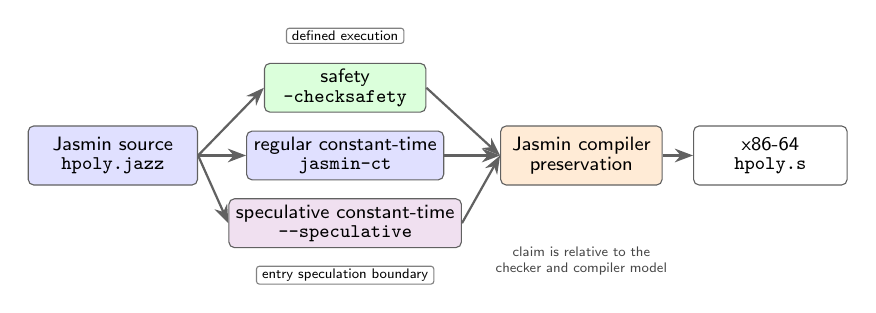
\begin{tikzpicture}[x=1cm,y=1cm]
  \node[vizbox, fill=vizPublic, minimum width=2.15cm] (src) at (0,0)
    {\jasmin{} source\\[-1pt]\texttt{hpoly.jazz}};
  \node[vizsmall, fill=vizSafety, minimum width=2.05cm] (safe) at (2.95,0.86)
    {safety\\[-1pt]\texttt{-checksafety}};
  \node[vizsmall, fill=vizPublic, minimum width=2.05cm] (ct) at (2.95,0)
    {regular \ct{}\\[-1pt]\texttt{jasmin-ct}};
  \node[vizsmall, fill=vizSct, minimum width=2.05cm] (sct) at (2.95,-0.86)
    {speculative \ct{}\\[-1pt]\texttt{--speculative}};
  \node[vizbox, fill=vizCompiler, minimum width=2.05cm] (comp) at (5.95,0)
    {\jasmin{} compiler\\[-1pt]preservation};
  \node[vizbox, fill=white, minimum width=1.95cm] (asm) at (8.35,0)
    {x86-64\\[-1pt]\texttt{hpoly.s}};

  \draw[vizarrow] (src.east) -- (safe.west);
  \draw[vizarrow] (src.east) -- (ct.west);
  \draw[vizarrow] (src.east) -- (sct.west);
  \draw[vizarrow] (ct.east) -- (comp.west);
  \draw[vizarrow] (safe.east) -- (comp.west);
  \draw[vizarrow] (sct.east) -- (comp.west);
  \draw[vizarrow] (comp.east) -- (asm.west);

  \node[viztag, fill=white] at (2.95,1.52) {defined execution};
  \node[viztag, fill=white] at (2.95,-1.52) {entry speculation boundary};
  \node[viznote] at (5.95,-1.34)
    {claim is relative to the\\checker and compiler model};
\end{tikzpicture}}
\caption{Compiler-side verification composition for the scalar \haetae{} NTT
artifact.  Safety, regular \ct{}, and SCT are checked on the same \jasmin{}
source; the compiler-preservation step connects those source-level facts to the
generated scalar assembly.}
\label{fig:verification-composition}
\end{figure}

\section{Implementation Target}

The artifact consists of five source/support files.  \path{params.jinc} fixes
the transform size and modulus; \path{reduce.jinc}
implements Montgomery reduction and field multiplication; \path{zetas.jinc}
contains the forward and inverse twiddle tables; \path{poly.jinc} contains the
stage-specialized kernels; and \path{hpoly.jazz} contains the exported ABI
wrappers.  Table~\ref{tab:files} summarizes the roles relevant to safety and
\ct{} verification.
The verification arguments below rely on the literal sizes in
\path{params.jinc}: every polynomial pointer has type
\texttt{u32[HAETAE\_N]}, every twiddle table has exactly 256 entries,
\(\texttt{HAETAE\_Q}=64513\), and \(\texttt{HAETAE\_N}=256\).

\begin{table}[t]
\centering
\scriptsize
\setlength{\tabcolsep}{3pt}
\begin{tabular}{P{0.30\columnwidth}P{0.60\columnwidth}}
\toprule
File & Verification-relevant role \\
\midrule
\path{params.jinc} & Shared constants \texttt{HAETAE\_Q}=64513 and
\texttt{HAETAE\_N}=256. \\
\path{hpoly.jazz} & Exported wrappers, \texttt{ct}/\texttt{sct} annotations, and
entry \texttt{\#init\_msf()} calls. \\
\path{poly.jinc} & Forward NTT, inverse NTT, inverse scaling, and base
multiplication loops. \\
\path{reduce.jinc} & Montgomery arithmetic over fixed-width words. \\
\path{zetas.jinc} & Fixed 256-entry forward and inverse twiddle tables. \\
\bottomrule
\end{tabular}
\caption{Source files used by the scalar safety and \ct{} checks.}
\label{tab:files}
\end{table}

\subsection{Algorithmic and Functional Context}

The implementation target is the negacyclic ring
\[
  R_q=\mathbb{Z}_q[X]/(X^{256}+1),\qquad q=64513,
\]
with the primitive \(512\)th root \(\zeta_0=426\) used by the HAETAE reference
NTT~\cite{HAETAE2022,Pollard1971}.  At the abstract field level, the forward
transform evaluates a polynomial at the odd powers of \(\zeta_0\), arranged in
bit-reversed order:
\[
  \widehat{p}[i]
    = \sum_{j=0}^{255}
      p[j]\cdot \zeta_0^{(2\operatorname{brev}_8(i)+1)j}.
\]
The inverse transform applies the corresponding inverse matrix and a factor
\(256^{-1}\).  The EasyCrypt development used by the companion functional
proof follows this full 256-point HAETAE transform, rather than the incomplete
128-point structure used by MLKEM/Kyber.

The \jasmin{} tables are concrete Montgomery-word realizations of this
mathematics~\cite{Montgomery1985}.  The forward table slot 0 is padding; slots
1--255 contain signed Montgomery representatives of
\(\zeta_0^{\operatorname{brev}_8(k)}\).  The inverse table stores the inverse
butterfly constants explicitly in slots 0--254 and reserves slot 255 for the
final scale, the signed Montgomery word \(-29720\), representing
\(256^{-1}R^2\bmod q\) for \(R=2^{32}\).  The paper's safety and timing claims
therefore apply to the concrete table layout actually read by the scalar
source, while the EasyCrypt functional theorem supplies the separate link to
the abstract transform for the forward and inverse wrappers.

The public wrappers in \path{hpoly.jazz} expose three pointer-based procedures.
The suffix \texttt{p} is used consistently for pointer arguments: \texttt{rp}
is the result polynomial pointer, while \texttt{ap} and \texttt{bp} are the two
source polynomial pointers for base multiplication.  The base-multiplication
wrapper marks the source pointers as \texttt{const}; the destination pointer is
mutable.

\newpage
\begin{lstlisting}[caption={Exported wrapper shape in \texttt{hpoly.jazz}.},label={lst:wrappers}]
#[ct = "rp -> rp"]
#[sct = "{ ptr: transient, val: secret } -> { ptr: public, val: secret }"]
export
fn poly_ntt_jazz(reg mut ptr u32[HAETAE_N] rp) -> reg ptr u32[HAETAE_N] {
  _ = #init_msf();
  rp = _poly_ntt(rp);
  return rp;
}

#[ct = "rp -> rp"]
#[sct = "{ ptr: transient, val: secret } -> { ptr: public, val: secret }"]
export
fn poly_invntt_jazz(reg mut ptr u32[HAETAE_N] rp) -> reg ptr u32[HAETAE_N] {
  _ = #init_msf();
  rp = _poly_invntt(rp);
  return rp;
}

#[ct = "rp * ap * bp -> {ap, bp, rp}"]
#[sct = "
{ ptr: transient, val: secret } *
{ ptr: transient, val: secret } *
{ ptr: transient, val: secret } ->
{ ptr: public, val: secret }
"]
export
fn poly_basemul_jazz(reg mut ptr u32[HAETAE_N] rp,
                     reg const ptr u32[HAETAE_N] ap bp) -> reg ptr u32[HAETAE_N] {
  _ = #init_msf();
  rp = _poly_basemul(rp, ap, bp);
  return rp;
}
\end{lstlisting}

The wrapper code is intentionally thin.  It does not perform arithmetic itself;
it establishes the security boundary and then calls an internal kernel.  This
separation is useful for verification.  The exported function is where the
caller-provided pointer enters the checked code, so this is where the
\texttt{sct} contract and \texttt{\#init\_msf()} appear.  The internal kernels
then run under the simpler invariant that pointer bases are public address
bases and coefficient values are secret data.

\subsection{Jasmin Implementation Discipline}

\jasmin{} is used here as a structured assembly language rather than as a
high-level source language.  The code makes the machine-level objects that
matter to verification explicit: register variables are declared with
\texttt{reg}, caller-provided arrays are typed as \texttt{ptr u32[HAETAE\_N]},
and mutability is visible at the function boundary.  A declaration such as
\[
  \texttt{reg mut ptr u32[HAETAE\_N] rp}
\]
is therefore more than documentation.  It gives the checker a typed 256-word
shape for indexed accesses through \texttt{rp}, tells the compiler that the
pointer is passed in a register, and records that the routine may write through
the pointer.  It does not by itself allocate or validate memory: the initial
state must still provide a valid, aligned region satisfying the pointer
precondition.  The source pointers of \path{poly_basemul_jazz} are instead
\texttt{reg const ptr u32[HAETAE\_N]}, which matches the implementation
discipline that \texttt{ap} and \texttt{bp} are read-only inputs.

The \jasmin{} documentation explains the source structure used by this artifact:
programs are assembled from \texttt{require}d files, parameters, global
variables, type aliases, and functions.  This is exactly the organization in
Table~\ref{tab:files}.  The constants in \path{params.jinc} are parameters, so
they may appear in array sizes such as \texttt{u32[HAETAE\_N]} and are resolved
early by the compiler.  The twiddle tables in \path{zetas.jinc} are global
arrays stored in immutable code memory.  The array documentation also explains
why the implementation introduces \texttt{reg ptr u32[256] zetasp} before
reading \path{jzetas}: a \texttt{reg ptr} is the Jasmin idiom for holding the
address of a global array or caller-provided array in a register.

Array indexing has the usual zero-based meaning, but the index is implicitly
scaled by the declared element size.  Thus \texttt{rp[idx]} denotes the
\texttt{u32} cell at byte offset \(4\cdot\texttt{idx}\) from the public base
address \texttt{rp}.  This matters to both safety and timing.  Safety needs
\(\texttt{idx}<256\), not merely a byte offset bound, while the timing checker
sees that the emitted address is a public base plus a public scaled index.  The
code avoids register arrays with run-time indices, which the manual warns must
be statically known after inlining and unrolling.  Instead, the polynomial and
table objects are memory arrays, for which run-time public indices are the
intended use case.  The 2026 \jasmin{} material also records newer register
spilling support, including auto-spill modes, but this artifact does not rely on
those features: it is compiled with the ordinary command line recorded in
Section~\ref{sec:evidence}.

The scalar-type documentation is also relevant.  Coefficients are machine words
(\texttt{u32}), whose arithmetic is the usual wrapping word arithmetic.  Loop
and index variables are word-sized integers (\texttt{ui64}), which behave like
bounded mathematical integers in the source semantics and are compiled to
machine words later.  Operations producing such values carry range assertions:
if a \texttt{ui64} computation overflowed its source-level range, execution
would be stuck and the safety checker would have to reject the program.  In this
implementation, the small stage counters and offsets make those range
assertions straightforward.

The NTT kernels avoid features that would make the low-level reasoning
unnecessarily indirect.  They allocate no source-level arrays, perform no raw
byte-addressed loads such as \texttt{[p + e]}, use no recursion, and call only
small arithmetic helpers whose effects are visible in the same \jasmin{} source
unit.  The observable memory operations are therefore precisely the typed
polynomial accesses, the typed twiddle-table accesses, and the final stores
back to the result polynomial.  This is why the proof obligations can be read
from the source: every address is a base pointer plus a public word index, and
every non-address data dependency is coefficient arithmetic in registers.

The implementation also separates the public NTT schedule from the secret data
flow.  The usual in-place butterfly for a stage of length \(\ell\) reads two
cells \(r_i\) and \(r_{i+\ell}\), computes a Montgomery product
\(t=\zeta r_{i+\ell}\), and writes \(r_i+t\) and \(r_i-t\) back to the same two
publicly determined positions.  In the \jasmin{} code the schedule variables
\texttt{block}, \texttt{j}, \texttt{start}, \texttt{idx}, and
\texttt{offset} are public loop counters or expressions built from them.  The
variables \texttt{s}, \texttt{coeff}, and \texttt{t} carry coefficient values
and are allowed to be secret.  The code is therefore arranged so that the
checker sees a syntactic separation between the public schedule and the secret
arithmetic payload.

\begin{figure}[t]
\centering
\resizebox{\columnwidth}{!}{%
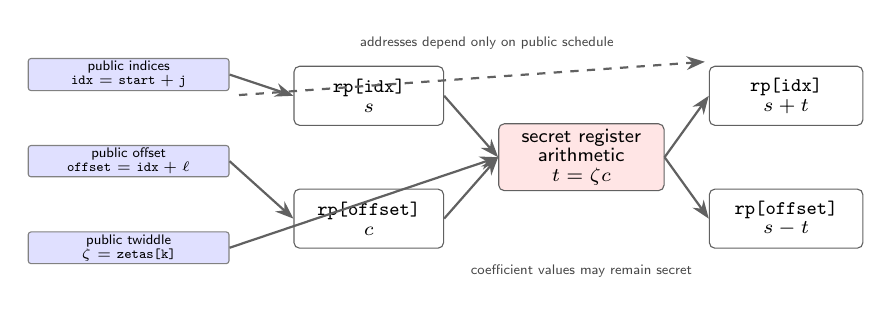
\begin{tikzpicture}[x=1cm,y=1cm]
  \node[viztag, fill=vizPublic, minimum width=2.55cm] (idx) at (0,1.05)
    {public indices\\[-1pt]\(\texttt{idx}=\texttt{start}+\texttt{j}\)};
  \node[viztag, fill=vizPublic, minimum width=2.55cm] (off) at (0,-0.05)
    {public offset\\[-1pt]\(\texttt{offset}=\texttt{idx}+\ell\)};
  \node[viztag, fill=vizPublic, minimum width=2.55cm] (tw) at (0,-1.15)
    {public twiddle\\[-1pt]\(\zeta=\texttt{zetas[k]}\)};

  \node[vizbox, fill=white, minimum width=1.9cm] (mem1) at (3.05,0.78)
    {\texttt{rp[idx]}\\[-1pt]\(s\)};
  \node[vizbox, fill=white, minimum width=1.9cm] (mem2) at (3.05,-0.78)
    {\texttt{rp[offset]}\\[-1pt]\(c\)};
  \node[vizbox, fill=vizSecret, minimum width=2.1cm] (arith) at (5.75,0)
    {secret register\\[-1pt]arithmetic\\[-1pt]\(t=\zeta c\)};
  \node[vizbox, fill=white, minimum width=1.95cm] (out1) at (8.35,0.78)
    {\texttt{rp[idx]}\\[-1pt]\(s+t\)};
  \node[vizbox, fill=white, minimum width=1.95cm] (out2) at (8.35,-0.78)
    {\texttt{rp[offset]}\\[-1pt]\(s-t\)};

  \draw[vizarrow] (idx.east) -- (mem1.west);
  \draw[vizarrow] (off.east) -- (mem2.west);
  \draw[vizarrow] (tw.east) -- (arith.west);
  \draw[vizarrow] (mem1.east) -- (arith.west);
  \draw[vizarrow] (mem2.east) -- (arith.west);
  \draw[vizarrow] (arith.east) -- (out1.west);
  \draw[vizarrow] (arith.east) -- (out2.west);

  \draw[vizdash] ($(idx.south east)+(0.12,-0.05)$) -- ($(out1.north west)+(-0.05,0.05)$);
  \node[viznote] at (4.55,1.45)
    {addresses depend only on public schedule};
  \node[viznote] at (5.75,-1.45)
    {coefficient values may remain secret};
\end{tikzpicture}}
\caption{One butterfly instance as seen by the safety and \ct{} checks.  The
public loop schedule determines the two addressed cells and the twiddle-table
entry, while coefficient-dependent values stay in register arithmetic and stored
data.}
\label{fig:butterfly-flow}
\end{figure}

Stage specialization is the main implementation device used to make this
separation automatic-checker friendly.  A compact C-style NTT loop would carry
a mutable \texttt{len} variable and would require the checker to relate
\texttt{len}, \texttt{start}, \texttt{j}, and table offsets across nested loops.
The \jasmin{} artifact instead expands the eight stages into eight helpers.
Each helper has literal loop bounds and literal offsets, so the checker sees
ordinary integer facts such as \(\texttt{block}<4\), \(\texttt{j}<32\), and
\(\texttt{offset}=\texttt{start}+\texttt{j}+32\).  This does not change the NTT
algorithm; it changes the presentation of the program so that the safety and
timing invariants are local to each helper.

\subsection{Montgomery Arithmetic Layer}

The arithmetic layer in \path{reduce.jinc} follows the C reference convention
for \haetae{}.  The constant \texttt{QINV} is \(q^{-1}\bmod 2^{32}\), with
\(q=64513\).  The reduction procedure first truncates the input to 32 bits,
multiplies by \texttt{QINV} with wrapping 32-bit semantics, sign-extends that
word, subtracts the corresponding multiple of \(q\), and performs an
arithmetic right shift by 32 bits.  The \jasmin{} code makes each width change
explicit:
\newpage
\begin{lstlisting}[caption={Montgomery arithmetic in \texttt{reduce.jinc}.},label={lst:reduce}]
inline fn __montgomery_reduce(reg u64 a) -> reg u32 {
  reg u32 t32;
  reg u64 t64;

  t32 = (32u)a;
  t32 *= QINV;
  t64 = (64s)t32;
  t64 *= HAETAE_Q;
  a   -= t64;
  a >>s= 32;
  t32  = (32u)a;
  return t32;
}

inline fn __fqmul(reg u32 a b) -> reg u32 {
  reg u64 ta tb t;
  reg u32 r;

  ta = (64s)a;
  tb = (64s)b;
  t  = ta * tb;
  r  = __montgomery_reduce(t);
  return r;
}
\end{lstlisting}

This layer is important for the \ct{} argument.  Coefficients and products are
secret, but the operations in Listing~\ref{lst:reduce} are arithmetic
operations on registers.  They do not choose an instruction path and they do
not compute a memory address.  The \jasmin{} x86 checker therefore needs to
accept the selected arithmetic instructions under its constant-time instruction
model, while still forbidding the same secret values from reaching branches or
addresses.

\subsection{Forward Transform}

The forward transform is written as eight fixed helpers.  The wrapper
\path{_poly_ntt} calls them in descending stage-length order:
\[
  128,64,32,16,8,4,2,1.
\]
Each helper fixes a pointer \texttt{zetasp} to the forward table
\path{jzetas}, iterates over a public block counter, loads a public
twiddle-table entry, and then performs a public inner loop over the butterflies
in that block.  The first helper illustrates the pattern:
\newpage
\begin{lstlisting}[caption={First stage-specialized forward NTT helper.},label={lst:nttstage}]
fn _poly_ntt_stage_128(reg mut ptr u32[HAETAE_N] rp)
    -> reg ptr u32[HAETAE_N] {
  reg ptr u32[256] zetasp;
  reg ui64 block j start idx offset;
  reg u32 zeta t s coeff;

  zetasp = jzetas;
  block = 0;
  while (block < 1) {
    zeta = zetasp[1 + block];
    start = block;
    start <<= 8;
    j = 0;
    while (j < 128) {
      idx = j;
      idx += start;
      s = rp[idx];
      offset = idx;
      offset += 128;
      coeff = rp[offset];
      t = __fqmul(zeta, coeff);
      coeff = s;
      coeff -= t;
      rp[offset] = coeff;
      s += t;
      rp[idx] = s;
      j += 1;
    }
    block += 1;
  }
  return rp;
}
\end{lstlisting}

Two details make this code friendly to the automatic checker.  First, all
indices are unsigned 64-bit loop variables or expressions built from them.
Second, the stage length appears as a literal in the helper: the checker sees
\texttt{block < 1}, \texttt{j < 128}, and \texttt{offset = idx + 128} in the
first helper, rather than having to infer a relation between a mutable
\texttt{len} variable and several nested loops.  The later helpers instantiate
the same proof shape with \texttt{block < 2}, \texttt{j < 64};
\texttt{block < 4}, \texttt{j < 32}; and so on.  This is not an algorithmic
change relative to the direct Cooley--Tukey schedule; it is an implementation
choice that exposes the public stage constants to \texttt{jasminc}.

\subsection{Inverse Transform and Final Scale}

The inverse transform mirrors the same implementation strategy in the opposite
stage order.  It starts at length 1 and ends at length 128, then applies a
separate final scaling loop.  The inverse helpers read from
\path{jzetas_inv}; their table bases are literal offsets
\[
  0,128,192,224,240,248,252,254.
\]
The final scale reads \path{jzetas_inv[255]} and multiplies every coefficient
by that fixed factor.  Treating the final scale as a separate helper keeps both
the safety and timing arguments simple: its only index is the public loop
counter \texttt{j}, with guard \texttt{j < HAETAE\_N}.

The inverse butterfly also has no data-dependent control.  It reads
\texttt{rp[idx]} and \texttt{rp[offset]}, computes the sum and Montgomery-scaled
difference, and stores both results back.  The arithmetic values are secret,
but the pair of touched locations is determined solely by the public stage
length, public block counter, and public inner-loop counter.

\subsection{Base Multiplication}

The base-multiplication kernel is the simplest example of the memory discipline:
it performs a public 256-iteration loop, reads one word from each source
polynomial, computes a Montgomery product, and writes one word to the result
polynomial.

\begin{lstlisting}[caption={Base multiplication in \texttt{poly.jinc}.},label={lst:basemul}]
fn _poly_basemul(reg mut ptr u32[HAETAE_N] rp,
                 reg const ptr u32[HAETAE_N] ap bp) -> reg ptr u32[HAETAE_N] {
  reg ui64 i;
  reg u32 a b r;

  i = 0;
  while (i < HAETAE_N) {
    a = ap[i];
    b = bp[i];
    r = __fqmul(a, b);
    rp[i] = r;
    i += 1;
  }
  return rp;
}
\end{lstlisting}

\section{Jasmin Verification Model}

\jasmin{} was designed to give programmers assembly-level control while keeping
source-level verification tractable~\cite{Jasmin2017,LastMile2020}.  The 2026
framework material is the current baseline used here: it presents \jasmin{} as
a predictable structured-assembly language, stresses source-level safety and
\ct{} checks, and states the information-flow rule that branch conditions and
memory indices must be public~\cite{JasminFramework2026}.  The older papers and
slides give the theoretical and instrumental background; the 2026 slides fix
the terminology and tool expectations used in this paper
~\cite{JasminWorkshop2021,JasminWorkbench2023,JasminCourse2024}.

The two core principles are unchanged.  Safety is a definedness property: every
memory access must be valid, every array index must be in bounds, and primitive
operations must be used within their semantic domains.  \ct{} security is a
trace property: two executions that agree on public inputs must produce the same
sequence of branches and memory read/write operations, even if their secret
state differs.

\subsection{Theoretical Foundation}

The theoretical basis used in this paper is layered.  The original \jasmin{}
work gives the language a machine-checked semantics, provides source analyses
for safety and \ct{}, and proves that the compiler preserves source behavior and
\ct{} under its model~\cite{Jasmin2017}.  The Last Mile work extends this
view into a methodology for developing optimized cryptographic implementations:
write code in \jasmin{}, prove or check source-level functional and
implementation-security properties, then rely on the predictable verified
compiler to connect those properties to assembly~\cite{LastMile2020}.  The
2021 and 2023 Jasmin workbench material presents the same separation in tool
form: safety checking, EasyCrypt extraction for functional reasoning, and
explicit leakage traces for implementation security
~\cite{JasminWorkshop2021,JasminWorkbench2023}.  The 2024--2026 course material
is the current standard adopted here: it distinguishes functional correctness
(including safety), implementation security, and cryptographic-security
reductions; it also records the current safety-checking workflow and the source
information-flow rule that branch conditions and memory indices must be public
~\cite{JasminCourse2024,JasminFramework2026}.

This layered reading also fixes what each local claim can and cannot mean.  The
Kyber implementation-correctness paper shows how Jasmin and EasyCrypt have been
used for lattice NTTs: finite-field representation, twiddle-table schedules,
bit-reversal, and optimized loop orders are handled by intermediate programs and
relational proofs, while implementation-security checks remain a separate layer
~\cite{KyberVerify2023}.  That precedent supports the division used here: this
paper proves safety and timing properties of the HAETAE scalar NTT source, while
functional NTT correctness belongs to the companion EasyCrypt development.
Likewise, the recent compiler-security paper formalizes a stronger but different
question, namely preservation of cryptographic security experiments for the
Jasmin compiler front-end using interaction trees and RHL
~\cite{ArranzOlmos2025JasminSecurity}.  It is cited to position the work, not as
an unstated proof of HAETAE signature security, compiler back-end security, or
side-channel security for this artifact.

\begin{table}[t]
\centering
\scriptsize
\setlength{\tabcolsep}{3pt}
\begin{tabular}{P{0.35\columnwidth}P{0.55\columnwidth}}
\toprule
Source family & Role in this paper \tabularnewline
\midrule
\jasmin{} CCS and Last Mile papers & Formal semantics, checked source
properties, predictable verified compilation, and source-to-assembly \ct{}
preservation. \tabularnewline
2021--2026 \jasmin{} slides & Current tool interpretation: old versus modular
safety checking, explicit CT annotations, EasyCrypt extraction, and the 2026
framework terminology. \tabularnewline
Spectre/SCT material & Three-level \texttt{secret}/\texttt{public}/
\texttt{transient} typing, MSF discipline, \texttt{\#init\_msf()} lowering, and
the Spectre-v1 scope of SCT~\cite{JasminSpectre2022,JasminCourse2024}.
\tabularnewline
Kyber implementation-correctness paper & NTT proof precedent separating
field-level functional correctness from implementation safety and timing
claims. \tabularnewline
2025 compiler-security paper & Boundary marker for cryptographic-security
preservation; complementary to this artifact-level safety/CT/SCT result.
\tabularnewline
\bottomrule
\end{tabular}
\caption{How the non-main dissertation PDFs support the theory used here.}
\label{tab:theory-sources}
\end{table}

\subsection{Threat and Leakage Model Used Here}


The implementation-level adversary considered here observes the leakage trace
modeled by the \jasmin{} x86 checkers, not arbitrary physical side channels.
The public inputs are the selected routine, pointer bases, loop bounds, table
layout, stage constants, and fixed twiddle-table locations.  The secret state is
the polynomial coefficient data and every arithmetic value derived from those
coefficients.  The regular \ct{} check treats branch decisions, loop guards,
memory addresses, array indices, and non-\ct{} instruction operands as
observable.  The intended invariant is therefore precise: changing the
coefficients may change register values and stored coefficient values, but must
not change the executed control-flow path or the sequence of memory locations
touched by the program.

The speculative checker extends this model in the \jasmin{}
\sct{}/Spectre-v1-style sense used by the tool.  Exported wrappers receive
transient pointer inputs and fence the boundary before calling the internal
kernels; inside the kernels, pointer bases and indices are public while loaded
coefficient values remain secret.  This is a model-relative statement.  It does
not claim coverage of every microarchitectural channel, such as power,
electromagnetic leakage, frequency effects, replacement-policy state, or
prefetch behavior not represented by the checker.  It also does not remove the
ordinary ABI precondition that the caller passes valid, aligned polynomial
regions.

\subsection{Principle of the Safety Check}

The safety checker is an abstract interpreter for the \jasmin{} source
semantics.  It does not prove that the NTT computes the right polynomial
transform; it proves that the program never steps outside the semantic domain
assumed by such a functional proof.  For this artifact, the important safety
preconditions come from the exported types: a caller must pass valid 256-word
\texttt{u32} regions for the polynomial pointers, and the global twiddle tables
must have the declared 256-entry layout.  Under those preconditions, the checker
generates and discharges local obligations for each command.

The manual description of \texttt{-checksafety} is useful for interpreting the
output.  The flag checks the safety of exported functions rather than simply
emitting assembly, and the reported result is conditional on a safety
precondition for the initial state.  The documented notion of safety includes
termination, in-bounds array accesses, valid and properly aligned allocated
memory, and valid arguments to arithmetic operations.  Thus
\texttt{No Safety Violation} for \path{poly_ntt_jazz} should be read as follows:
assuming the ABI supplies a valid aligned polynomial region for \texttt{rp}, all
calls reached from that export terminate without undefined \jasmin{} behavior.
The same reading applies to \path{poly_invntt_jazz} and
\path{poly_basemul_jazz}, with the latter adding valid aligned input regions
for \texttt{ap} and \texttt{bp}.

The 2026 \jasmin{} slides distinguish this command from a newer modular safety
workflow based on contracts, source assertions, automatic discharge, and
EasyCrypt proofs for remaining assertions~\cite{JasminFramework2026}.  This
paper intentionally uses \texttt{jasminc -checksafety}: the scalar NTT has no
symbolic heap structure, no source stack arrays, and no data-dependent loop
bounds, and the stage-specialized helpers expose exactly the small arithmetic
facts that the old static checker can discharge.  The successful run is
therefore evidence about this concrete artifact, not a claim that the old
checker is the preferred method for every modern \jasmin{} program.

The most visible obligations are array bounds and memory validity.  For an
access \texttt{rp[idx]}, the checker must know that \texttt{rp} denotes a valid
typed region and that the current abstract state entails
\(0 \leq \texttt{idx} < 256\).  For a store \texttt{rp[offset] = coeff}, it must
prove the same bound for \texttt{offset} and must also know that the pointer is
mutable.  The checker also tracks definedness of word-level operations: casts,
signed and unsigned interpretations, shifts, multiplications, and calls to
helpers must all be used in the way the \jasmin{} semantics permits.  Thus a
successful safety run should be read as a conditional statement: if the ABI
caller supplies valid typed regions, every source execution of the checked
routine is defined and every memory access stays inside its declared object.

This is the right safety principle for the scalar NTT because the code's memory
shape is simple.  The checker is not required to reason about alias-free heap
allocation, symbolic byte offsets, or data-dependent loop termination.  It only
has to propagate public counter ranges through the stage-specialized loops and
through the table-index expressions.  The resulting proof obligations are small
integer facts, and their connection to the source code is visible in each
helper's literal loop bounds.

\subsection{Principle of Constant-Time Verification}

The regular \ct{} checker is an information-flow analysis for the leakage trace
of the program.  The programmer supplies a security signature for each exported
function.  The checker then propagates labels through expressions and commands.
Values marked secret may be computed, combined, and stored; secrecy is not an
error by itself.  The error condition is a secret dependency reaching something
that the leakage model treats as observable: a branch condition, a loop guard,
a memory address, an array index, or an instruction operand that the selected
architecture model does not classify as constant time.

The \jasmin{} documentation and the recent slides distinguish two
constant-time methodologies: the
largely automatic type-system check used by \texttt{jasmin-ct}, and more
expressive proof-oriented methods for broader probabilistic notions.  This
artifact uses the automatic checker.  Its documented rules are exactly the ones
needed by the scalar NTT.  Constants are public; the label of an arithmetic
expression is the maximum of the labels of its operands; array indices and raw
memory addresses must be public; \texttt{if} and \texttt{while} conditions must
be public; and exported functions must carry explicit \texttt{ct} signatures
unless inference is requested for development.  The code uses no
\texttt{\#declassify} escape hatch, so the proof does not rely on an unverified
claim that a secret-derived value has become public
~\cite{JasminWorkbench2023,JasminFramework2026}.

This gives a precise meaning to the common implementation rule ``do not branch
or index on secrets.''  In the NTT code, polynomial coefficients are secret and
twiddle values are public table constants.  A coefficient may flow through
\texttt{\_\_fqmul}, additions, subtractions, casts, and stores.  It may not flow
into \texttt{j < 128}, into \texttt{1 + block}, into \texttt{idx}, or into
\texttt{offset}.  If it did, the checker would reject the program because two
runs with different coefficients could take different control paths or touch
different addresses.  Conversely, the public loop counters and fixed stage
constants are allowed to determine both branches and addresses.

The speculative checker strengthens this principle at exported boundaries.  The
documentation and the 2024--2026 slides present this as selective speculative
load hardening for Spectre v1-style transient execution
~\cite{JasminCourse2024,JasminFramework2026}.  Its key idea is that
cryptographic code already knows which values are public and which are secret,
so the hardening discipline can focus on public loads and pointer values whose
transient behavior must be controlled.  The SCT type system separates the
security of a pointer value from the security of the memory value reached
through that pointer and distinguishes normal execution from transient
execution.  A transient pointer is
architecturally public but is not treated as freely public for speculative
addressing until the misspeculation-flag state has been initialized.  The
manual states that exported-function arguments are treated at least as
\texttt{transient}, because an export cannot receive an MSF argument and the
compiler defensively assumes that execution may already be misspeculating at
entry.  The wrappers in Listing~\ref{lst:wrappers} therefore call
\texttt{\#init\_msf()} before entering the arithmetic kernels.  In the documented
x86 lowering, this operation emits an \texttt{lfence} and initializes the MSF to
the exact state.  After that boundary, the checker may type the pointer bases as
public while continuing to type the pointed-to polynomial coefficients as
secret.  The resulting claim is model-relative: it is evidence in the
\jasmin{} SCT checker's Spectre-v1-style leakage model for this source and call
graph, not a measurement claim and not a proof against every speculative or
microarchitectural channel.

The discussion here is grounded in portable artifact components rather than in
machine-specific paths.  The implementation is under \path{jasmin/}; the raw
reproduction logs are under \path{paper/logs/}; and the \jasmin{}
documentation pages used to interpret the tools are identified by their
source-tree-relative names:
\path{source/tools/safety_checker.md}, \path{source/tools/ct.md},
\path{source/tools/sct.md}, \path{source/language/semantics/arrays.md},
\path{source/language/semantics/scalar_types.md}, and
\path{source/compiler/passes/index.md}.  The commands below were reproduced
with repository revision \texttt{f0e1399} and \jasmin{} compiler version
\texttt{2026.03.0}.  The checker components in
Table~\ref{tab:checkerfiles} are likewise named relative to a \jasmin{} source
checkout or artifact container.  This matters because the paper does not ask
the reader to accept a folklore description of \jasmin{} verification: the
manual describes the intended tool interfaces, and the compiler source contains
the security annotation language, export-function annotation checks, and
speculative pointer/value type discipline.

\begin{table}[t]
\centering
\scriptsize
\setlength{\tabcolsep}{3pt}
\begin{tabular}{P{0.38\columnwidth}P{0.52\columnwidth}}
\toprule
Jasmin component & Role in this paper \\
\midrule
\path{compiler/safetylib} & Abstract-interpretation infrastructure
used by \texttt{jasminc -checksafety}. \\
\path{compiler/src/securityAnnotations.ml} & Parser for
\texttt{ct}/\texttt{sct} signatures, including named CT levels, arrows,
products, \texttt{transient}, and pointer/value SCT types. \\
\path{compiler/src/ct_checker_forward.ml} & Regular \ct{} checker;
exported functions must be fully annotated unless inference is requested, and
result labels must be justified by input labels. \\
\path{compiler/src/sct_checker_forward.ml} & Speculative checker;
models direct and indirect security types, enforces export-boundary
constraints, and handles the MSF discipline used by \texttt{\#init\_msf()}. \\
\path{compiler/entry/jasmin_ct.ml} & Command-line entry point for
\texttt{jasmin-ct} and \texttt{jasmin-ct --speculative}. \\
\bottomrule
\end{tabular}
\caption{\jasmin{} checker components used to interpret the artifact.}
\label{tab:checkerfiles}
\end{table}

The annotation parser explains the notation in Listing~\ref{lst:wrappers}.
For regular \ct{} contracts, an input type can be public, secret, unspecified,
or a named level such as \texttt{rp}, \texttt{ap}, or \texttt{bp}.  An output
type may mention a set of such input levels.  Thus
\texttt{rp * ap * bp -> \{ap, bp, rp\}} is not a mathematical product over
polynomials; it is a security signature saying that the returned value may
depend on the security levels assigned to the three input arguments.  For
speculative contracts, \path{securityAnnotations.ml} defines indirect types of
the form \(\{\texttt{ptr}:\ell_p,\texttt{val}:\ell_v\}\).  It also defines
\texttt{transient} as the level whose normal component is public and whose
speculative component is secret.  That is precisely the entry type used by the
exported wrappers.

The present implementation uses a small and regular subset of the \jasmin{}
memory model.  The source has no raw memory expression of the form
\texttt{[p + e]} and no source-level stack array.  Its observable source memory
operations are typed array and pointer operations:
\[
  \texttt{rp[idx]},\quad \texttt{rp[offset]},\quad
  \texttt{ap[i]},\quad \texttt{bp[i]},
\]
plus reads from the fixed global tables \path{jzetas} and \path{jzetas_inv}.
Thus the byte-block memory obligations from the general \jasmin{} model
specialize to word-array obligations: each caller-provided polynomial pointer
must designate a valid 256-word \texttt{u32} region, and every computed index
must lie in \([0,256)\).

The \ct{} checks are relative to the \jasmin{} x86 leakage model.  Branches and
memory addresses are observable.  Arithmetic instructions that the model
classifies as constant time do not add secret-dependent leakage obligations.
This distinction is important for this code.  Montgomery multiplication lowers
to arithmetic such as \texttt{imul} and \texttt{sar} on coefficient-derived
registers.  The checker accepts this arithmetic under the selected x86 model,
but it would reject any use of the same coefficient-derived values in branch
conditions, loop bounds, memory indices, or operations marked non-\ct{} by the
architecture model.

\section{Why the Checks Are Convincing}

The verification argument is not a collection of informal coding conventions.
It is a composition of three explicit checks over the actual \jasmin{} source.
Each check corresponds to a semantic obligation, and each obligation rules out a
different way in which an implementation theorem could be misleading.

The intended theorem can be stated as a conditional noninterference claim.  Let
two calls to one exported routine satisfy the same public ABI inputs, the same
typed pointer-validity preconditions, and possibly different polynomial
coefficients in the pointed-to arrays.  If both calls are run through the
\jasmin{} semantics and then compiled by the \jasmin{} compiler, they follow the
same branch schedule and touch the same sequence of memory addresses.  They may
write different coefficient values, because those values are secret outputs, but
the observable control/address trace is independent of those values.  The
safety check supplies the defined-execution premise of this statement; the
regular \ct{} check supplies the trace-noninterference premise; the speculative
\ct{} check supplies the corresponding entry-boundary premise for transient
execution; and the compiler argument connects these source properties to the
generated x86-64 code.

The pieces of this composition should not be conflated.  The safety statement
comes from \texttt{jasminc -checksafety} and is conditional on valid initial
memory.  The branch/address timing statement comes from \texttt{jasmin-ct} and
the \jasmin{} compiler's \ct{} preservation discipline as presented in the
current framework material~\cite{JasminFramework2026}.  The speculative
statement comes from the separate SCT checker and its Spectre-v1-style model.
Recent work on cryptographic-security preservation for the \jasmin{} compiler
front-end is related and important, but it proves a different theorem for KEM
IND-CCA security and does not by itself instantiate a full HAETAE signature,
back-end, or side-channel theorem for this artifact
~\cite{ArranzOlmos2025JasminSecurity}.

This chain is persuasive only if the checker obligations align with the actual
program structure.  In this artifact they do.  Table~\ref{tab:obligations}
lists the verification obligations and the concrete source facts that discharge
them.  None of the obligations relies on a hidden algebraic property of the NTT
or on a probabilistic assumption about coefficient values.  They are structural
facts about loops, indices, pointer types, and the placement of arithmetic
operations.

\begin{table}[t]
\centering
\scriptsize
\setlength{\tabcolsep}{3pt}
\begin{tabular}{P{0.34\columnwidth}P{0.56\columnwidth}}
\toprule
Obligation & Concrete reason it holds in the artifact \\
\midrule
Polynomial accesses are in bounds &
Every exported polynomial pointer has type \texttt{ptr u32[256]}, and all
indices are public counters bounded by literal stage sizes. \\
Twiddle accesses are in bounds &
Forward stages use table entries 1--255; inverse stages use entries 0--254;
the final inverse scale uses entry 255. \\
Branches are public &
All loop guards compare public counters with constants such as 128, 64, or
\texttt{HAETAE\_N}. \\
Addresses are public &
Address expressions contain pointer bases, public counters, and literal stage
offsets, never coefficient-derived words. \\
Secret values remain allowed where needed &
Coefficients and Montgomery products flow through register arithmetic and
stores, which is exactly the intended secret-data path. \\
Exported speculative boundary is explicit &
Each exported wrapper calls \texttt{\#init\_msf()} before entering the kernel,
and the \texttt{sct} signature separates pointer security from pointed-to
value security. \\
\bottomrule
\end{tabular}
\caption{Checker obligations matched to source-level implementation facts.}
\label{tab:obligations}
\end{table}

\paragraph{Safety establishes defined execution.}
The command \texttt{jasminc -checksafety} invokes the safety analysis under
\path{compiler/safetylib}.  In particular,
\path{safetyInterpreter.ml} builds safety conditions for array accesses,
sub-array accesses, memory validity, word-operation side conditions, and return
conditions, then reports \texttt{No Safety Violation} only when the abstract
state entails those conditions.  This matters because \ct{} is normally a
property of traces of executions; if the program could go out of bounds or
execute an invalid primitive operation, the trace argument would be about the
wrong semantics.  Safety is therefore the first layer: it says that every trace
considered by the timing checker corresponds to a defined low-level execution
under the typed pointer preconditions.

For this artifact the generated safety obligations are simple enough to audit
against the code.  The only caller-provided memory regions are the polynomial
pointers \texttt{rp}, \texttt{ap}, and \texttt{bp}; the only global arrays are
the 256-entry twiddle tables.  The stage-specialized code makes all array
indices public affine expressions of bounded counters.  Consequently, the
safety checker is not being asked to discover a cryptographic invariant about
secret data.  It is checking arithmetic facts such as
\(\texttt{j}<128 \Rightarrow \texttt{j}+128<256\) in the first forward stage,
and \(\texttt{i}<256\) for \texttt{ap[i]}, \texttt{bp[i]}, and \texttt{rp[i]} in
base multiplication.

\paragraph{Regular \ct{} is enforced as information flow to the leakage trace.}
The regular checker in \path{ct_checker_forward.ml} is a type system for the
parts of the program that may affect the timing trace.  Its expression checker
has a public mode: when an expression is used as an array index, memory address,
\texttt{if} condition, \texttt{while} guard, or bound, the checker calls the
expression typing function with the requirement that the result be public.  For
operations classified as not constant time by the architecture model, the
checker similarly requires public operands.  Exported functions are required to
have complete security annotations unless inference is explicitly requested,
and result labels may mention only levels that appear in the input signature.

This gives a precise interpretation to the successful \texttt{jasmin-ct} run.
It does not merely say that a reviewer failed to notice a secret branch.  It
says that the checker traversed the program and proved that every expression
contributing to the leakage trace is public in the specified security
environment.  In the \haetae{} NTT code, the secret values are exactly the
loaded polynomial coefficients and the arithmetic values derived from them.
Those values flow through \texttt{+}, \texttt{-}, casts, Montgomery
multiplication, and stores.  They do not flow to loop guards, branch
conditions, or address expressions.  The checker enforces precisely that
separation.

\paragraph{Speculative \ct{} validates the exported boundary.}
The speculative checker in \path{sct_checker_forward.ml} strengthens the
regular property by distinguishing normal and speculative security levels and
by splitting pointer security from pointed-to-value security.  The local
annotation parser defines \texttt{transient} as normal-public but
speculative-secret.  Thus a wrapper argument of type
\[
  \{\texttt{ptr}:\texttt{transient},\ \texttt{val}:\texttt{secret}\}
\]
means that the pointer is architecturally public but is treated cautiously under
transient execution until the microarchitectural speculation state is
initialized.  The checker also tracks MSF state: \texttt{\#init\_msf()} is a
special operation in the SCT checker, and in the x86 lowering used here it
corresponds to an \texttt{lfence} at the exported entry point.

The successful \texttt{jasmin-ct --speculative} run therefore rules out a
specific false proof pattern.  The proof is not allowed to assume that an
ABI-provided pointer is safely public for speculative addressing before the
entry hardening point.  After \texttt{\#init\_msf()}, the bodies of
\path{_poly_ntt}, \path{_poly_invntt}, and \path{_poly_basemul} use public
pointer bases and public counters for addresses, while the values loaded from
the arrays remain secret.  This is exactly the policy required for exported
cryptographic routines.

\paragraph{The compiler argument connects source checks to assembly.}
The final step is preservation through compilation.  The \jasmin{} compiler is
designed for predictable low-level transformations and is accompanied by the
compiler-correctness development described in the \jasmin{} paper
and subsequent framework material
~\cite{Jasmin2017,LastMile2020,JasminFramework2026}.  The safety and timing
argument here uses that discipline:
the source-level fixed schedule may be lowered to branches and indexed memory
operands, but the compiler is not allowed to introduce table lookups indexed by
secret values or branches on secret-dependent ranges.  This design choice is
what makes the source-level checks meaningful evidence for the generated
\path{hpoly.s}.  The claim is not that arbitrary optimizing compilation would
preserve \ct{}; the claim is that this source is checked by the \jasmin{}
toolchain and compiled by the \jasmin{} compiler under its preservation model.

The composition used in this paper is therefore the following artifact theorem
schema.  First, \texttt{jasminc -checksafety} proves that the three exported
source routines have defined executions under their typed pointer preconditions.
Second, \texttt{jasmin-ct} proves that their branch and memory-address leakage
trace is independent of coefficient values.  Third,
\texttt{jasmin-ct --speculative} proves the same source against the
\jasmin{} SCT checker's transient-pointer model.  Fourth, \texttt{jasminc}
compiles that source to scalar x86-64 assembly, and the regenerated assembly is
byte-for-byte identical to the submitted \path{hpoly.s}.  The conclusion is
conditional on exactly these premises: the submitted assembly is the compiler
output of the checked source, and its safety and timing claim is the one
preserved by the \jasmin{} model.  It is not a separate binary-analysis theorem,
and it does not extend to hand-edited assembly.

\paragraph{Why this is persuasive for this implementation.}
The implementation is intentionally shaped so that the checked proof
obligations coincide with the informal cryptographic discipline.  There are no
data-dependent loops, no data-dependent conditionals, no raw source-level
pointer arithmetic, and no table lookup indexed by a coefficient.  The only
variables that influence addresses are public counters and literal stage
constants; the only variables that carry secrets are coefficients and
coefficient-derived arithmetic temporaries.  The checker outputs are therefore
not a black-box certificate for an opaque program.  They confirm an auditably
simple invariant: public schedule and public addresses, secret arithmetic
values.

\section{Safety Argument}

The safety proof rests on the fact that all memory locations are selected by
public counters with literal bounds.  For a forward stage of length \(\ell\),
the helper has the schematic form
\[
  \texttt{block}<\frac{256}{2\ell},\qquad
  \texttt{j}<\ell,\qquad
  \texttt{start}=\texttt{block}\cdot 2\ell,
\]
with
\[
  \texttt{idx}=\texttt{start}+\texttt{j},\qquad
  \texttt{offset}=\texttt{idx}+\ell.
\]
The checker therefore needs only local arithmetic to prove
\[
  0 \leq \texttt{idx}<256
  \quad\text{and}\quad
  0 \leq \texttt{offset}<256.
\]
The first forward helper is the extreme case: \(\texttt{block}<1\),
\(\texttt{j}<128\), and \(\texttt{offset}=\texttt{j}+128\).  The remaining
helpers instantiate the same shape for smaller stage lengths and more blocks.
The inverse helpers use the same address structure in reverse stage order.  The
final inverse scale loop has only the single obligation \(0\leq j<256\).

The twiddle-table accesses are fixed by construction.  The forward transform
uses \path{jzetas[1]} through \path{jzetas[255]}; the inverse butterfly stages
use \path{jzetas_inv[0]} through \path{jzetas_inv[254]}; and the inverse final
scale reads \path{jzetas_inv[255]}.  These are all inside the 256-entry table
types.

Base multiplication has an even simpler safety shape.  The public loop counter
\texttt{i} ranges from 0 to 255, and the only source-level memory operations are
\path{ap[i]}, \path{bp[i]}, and \path{rp[i]}.  Since the wrapper type gives all
three pointers type \texttt{ptr u32[HAETAE\_N]} and \(\texttt{HAETAE\_N}=256\),
the safety proof reduces to the loop-bound invariant \(0\leq i<256\).  The
\texttt{const} qualifier on \texttt{ap} and \texttt{bp} also matches the
intended data flow: the source polynomials are read, and only \texttt{rp} is
written.

\section{Constant-Time Argument}

The regular \ct{} checker enforces the CCS-style leakage discipline
syntactically.  Any expression that determines a branch, loop guard, memory
address, or array index must be public.  Coefficients and Montgomery products
may be secret, but they must not control the trace.

For the forward and inverse NTT, all coefficient-derived values stay in
arithmetic positions.  A loaded coefficient may be added, subtracted, cast,
shifted, or multiplied in Montgomery arithmetic, and the result may be stored
back to a polynomial cell.  It never flows into a branch condition, loop bound,
or address expression.  The loop schedule is fixed by stage constants, and the
twiddle-table indices are public expressions such as \(\texttt{1+block}\),
\(\texttt{64+block}\), or \(\texttt{254+block}\).

For base multiplication, the trace is the public 256-iteration load/load/store
pattern shown in Listing~\ref{lst:basemul}.  The loaded values \texttt{a} and
\texttt{b} are secret.  The product \texttt{r} is secret.  However, the branch
condition is \(\texttt{i}<256\), and every memory address uses the same public
index \texttt{i}.  Thus the coefficient values determine only the words written
to \texttt{rp}, not which instructions execute or which locations are touched.

The regular \texttt{ct} annotations on the exported wrappers record the
security dependency of results without forcing polynomial data to be public.
For \path{poly_ntt_jazz} and \path{poly_invntt_jazz}, the annotation
\texttt{rp -> rp} states that the returned pointer/result has the same security
dependence as the input polynomial argument.  For \path{poly_basemul_jazz}, the
annotation
\[
  \texttt{rp * ap * bp -> \{ap, bp, rp\}}
\]
uses \texttt{rp}, \texttt{ap}, and \texttt{bp} as named security levels.  The
result label is conservative: the returned pointer is allowed to depend on all
three input labels even though the source body returns the destination pointer.
The essential \ct{} obligation is separate from minimality of this label: the
checker still requires the indices in \path{ap[i]}, \path{bp[i]}, and
\path{rp[i]} to be public.

\section{Speculative Constant-Time}

The speculative checker strengthens the regular property for transient
execution.  The implementation uses \texttt{sct} annotations that distinguish a
pointer's security level from the security level of values reachable through the
pointer:
\[
  \{\texttt{ptr}:\ell_p,\ \texttt{val}:\ell_v\}.
\]
The exported wrappers accept transient pointers to secret polynomial values and
return public pointers to secret polynomial values.  Intuitively, the pointer
base is allowed to become public after the entry speculation boundary, while
the coefficients remain secret throughout.

The source instruction \texttt{\#init\_msf()} is the hardening boundary.  In the
checker it initializes the microarchitectural speculation state; in the x86-64
lowering used here, the exported assembly begins with an \texttt{lfence}.  After
that point, the NTT and base-multiplication bodies use only public pointer bases
and public counters for addressing.  Secret values loaded from polynomial cells
flow into arithmetic and stores, not into transient address computation.

This matters for the public ABI boundary.  A regular \ct{} proof would rule out
leaks from committed branches and committed addresses.  The speculative proof
also prevents the reasoning from silently assuming that a public-looking pointer
or bound remains public before the entry fence.  In this implementation there
are no secret-dependent bounds to harden inside the polynomial kernels; the only
required speculation boundary in the \jasmin{} SCT model for this call graph is
at the exported entry point.  This is not a claim about all speculative
execution variants, data-dependent prefetching, frequency effects, or other
microarchitectural channels outside that model.

\section{Compiler-Level Guarantee}

The checks above are run on \path{jasmin/hpoly.jazz}, not on a hand-written
assembly proof.  This is meaningful because \jasmin{} is designed around a
predictable compiler whose transformations preserve the source-level
discipline~\cite{Jasmin2017,LastMile2020,JasminFramework2026}.  The compiler
avoids optimizations that are
dangerous for \ct{} code, such as replacing secret arithmetic by table lookups
or introducing case splits on secret-dependent values.  Public loop structure
may be lowered into branches and indexed memory operands, but secret values must
not become branch predicates or address selectors.  Thus the formal claim is a
composition of source-level checker results with the \jasmin{} compiler's
preservation theorem and timing discipline; the assembly inspection below is a
sanity check that the generated code has the expected public-counter shape.

This paper does not use the newer front-end cryptographic-security
preservation theorem as a premise for HAETAE.  That theorem is cited as related
work on the gap between source-level cryptographic proofs and compiled code; it
is front-end-focused and KEM/IND-CCA-focused, whereas the present result is a
source-to-assembly safety and timing argument for scalar NTT kernels.

The generated scalar assembly has the expected shape.  Each exported wrapper
contains an entry \texttt{lfence}.  The base-multiplication body lowers
\path{ap[i]}, \path{bp[i]}, and \path{rp[i]} to base-plus-scaled-index memory
operands with the public loop counter as the scaled index, and the loop branch
compares that counter with the constant 256.  The NTT stage loops likewise
branch on public counters and form addresses from the public base pointer,
public stage constants, and public counters.  Coefficients appear in arithmetic
registers and stored words, but not in branch predicates or address registers.

The compiler-level guarantee should therefore be read as a conditional
composition: source-level safety, source-level \ct{} checks, speculative entry
hardening, and \jasmin{}'s preservation discipline together justify using the
generated assembly as the checked scalar implementation.  The claim is stronger
than a manual style audit of the assembly because the argument is tied to the
source contracts and compiler invariants, but it remains relative to the
\jasmin{} semantics, checker model, and compiler version identified in the
artifact.

\section{Verification Evidence}
\label{sec:evidence}

The commands in Table~\ref{tab:checks} were run on the artifact.  The safety
checker reports no safety violation for all three exported routines.  The
regular \ct{} checker exits successfully.  The speculative checker exits
successfully and prints the expected public-pointer/secret-value signatures for
the internal kernels and exported wrappers.

\begin{table}[t]
\centering
\scriptsize
\setlength{\tabcolsep}{3pt}
\begin{tabular}{P{0.50\columnwidth}P{0.40\columnwidth}}
\toprule
Command & Result \\
\midrule
\texttt{jasminc -checksafety -o /tmp/hpoly-safe.s jasmin/hpoly.jazz}
& No safety violation for \path{poly_ntt_jazz}, \path{poly_invntt_jazz}, and
\path{poly_basemul_jazz}. \\
\texttt{jasmin-ct jasmin/hpoly.jazz}
& Regular \ct{} check passed. \\
\texttt{jasmin-ct --speculative jasmin/hpoly.jazz}
& Speculative \ct{} check passed; exported wrappers have transient pointer
inputs and public pointer, secret value outputs. \\
\bottomrule
\end{tabular}
\caption{Compiler-side verification evidence.}
\label{tab:checks}
\end{table}

For reproducibility, the reported run used \texttt{jasminc -version} =
\texttt{Jasmin Compiler 2026.03.0} and repository revision \texttt{f0e1399}.
The raw logs are included in \path{paper/logs/}: \path{jasminc-version.log},
\path{git-revision.log}, \path{jasmin-checksafety.log},
\path{jasmin-ct.log}, \path{jasmin-ct-speculative.log}, and
\path{jasmin-compile.log}.  The generated assembly from
\texttt{jasminc jasmin/hpoly.jazz -o /tmp/hpoly-after.s} was byte-for-byte
identical to the checked \path{hpoly.s}; the artifact records this through
\path{assembly-sha256.log} and the empty \path{assembly-diff.log}.  A submitted
artifact should also identify the exact \jasmin{} compiler source or container
image, because the safety and timing claims are relative to the checker
implementation used for these commands.

Table~\ref{tab:raw-evidence} summarizes the reviewer-facing evidence that was
checked against the raw logs and generated assembly.  The table is not a
substitute for the logs; it records which concrete artifacts support each
claim so that the paper remains auditable without relying on prose alone.

\begin{table}[t]
\centering
\scriptsize
\setlength{\tabcolsep}{3pt}
\begin{tabular}{P{0.35\columnwidth}P{0.55\columnwidth}}
\toprule
Artifact evidence & What it shows \\
\midrule
\path{jasmin-checksafety.log} &
All three exports report \texttt{No Safety Violation}; the base-multiplication
report names \texttt{mem\_rp}, \texttt{mem\_ap}, and \texttt{mem\_bp}. \\
\path{jasmin-ct-speculative.log} &
Internal kernels are typed with public pointer bases and secret values; exported
wrappers accept transient pointers and return public pointers to secret values. \\
\path{hpoly.s} &
Each exported wrapper begins with \texttt{lfence}; loops compare public
counters with constants and use base-plus-scaled-index memory operands. \\
\path{assembly-sha256.log}, \path{assembly-diff.log} &
The regenerated assembly and checked \path{hpoly.s} have identical SHA-256
hashes, and the recorded diff is empty. \\
\bottomrule
\end{tabular}
\caption{Raw evidence used to audit the checker and assembly claims.}
\label{tab:raw-evidence}
\end{table}

A minimal reproduction run from the repository root has four steps.  First,
record the tool and source versions with \texttt{jasminc -version} and
\texttt{git rev-parse --short HEAD}.  Second, run the three source checks:
\texttt{jasminc -checksafety -o /tmp/hpoly-safe.s jasmin/hpoly.jazz},
\texttt{jasmin-ct jasmin/hpoly.jazz}, and
\texttt{jasmin-ct --speculative jasmin/hpoly.jazz}.  Third, regenerate assembly
with \texttt{jasminc jasmin/hpoly.jazz -o /tmp/hpoly-after.s}.  Finally, compare
\path{hpoly.s} with the regenerated file, for example by SHA-256 and an ordinary
diff.  The expected result is exactly the one recorded in \path{paper/logs/}: no
safety violation, successful regular and speculative \ct{} checks, matching
assembly hashes, and an empty assembly diff.

\begin{table}[t]
\centering
\scriptsize
\setlength{\tabcolsep}{3pt}
\begin{tabular}{P{0.25\columnwidth}P{0.18\columnwidth}P{0.47\columnwidth}}
\toprule
Surface & Size & Checked role \\
\midrule
Constants and tables & 69 source lines &
\path{params.jinc} and \path{zetas.jinc} fix \(q\), \(n\), and the twiddle
layout used by the stage-specialized loops. \\
Arithmetic helpers & 34 source lines &
\path{reduce.jinc} supplies \texttt{\_\_montgomery\_reduce} and
\texttt{\_\_fqmul}; the check keeps their arithmetic results away from branches
and addresses. \\
Polynomial kernels & 698 source lines &
\path{poly.jinc} contains eight forward stages, eight inverse stages, final
scaling, and base multiplication. \\
ABI wrappers & 38 source lines &
\path{hpoly.jazz} exports the three checked routines and attaches the
\ct{}/\sct{} boundary annotations. \\
Generated assembly & 908 assembly lines &
\path{hpoly.s} contains the three exported wrappers, each with an entry
\texttt{lfence}, and the compiled stage loops. \\
Raw verification logs & 211 log lines &
\path{paper/logs/*.log} records the compiler version, source revision, checker
outputs, assembly hashes, and empty assembly diff. \\
\bottomrule
\end{tabular}
\caption{Artifact size and checked surface.  The table is an audit summary, not
a runtime benchmark.}
\label{tab:surface}
\end{table}

The table also defines when the evidence must be regenerated.  A change to
\path{hpoly.jazz}, \path{poly.jinc}, \path{reduce.jinc},
\path{zetas.jinc}, or \path{params.jinc} changes the checked source surface.  A
change to the \jasmin{} compiler version changes the checker implementation.  A
change to \path{hpoly.s} changes the assembly object whose fence placement and
memory-address discipline are being cited.  Any of these changes invalidates
the recorded evidence unless the safety, regular \ct{}, speculative \ct{}, and
assembly-comparison logs are regenerated.  Likewise, adding raw memory
operations, data-dependent branches, declassification, or new wrappers without
matching \ct{}/\sct{} signatures would require a fresh review of the leakage
argument, not only a rerun of the commands.

The safety output for base multiplication is particularly informative because
it names the three memory arguments:
\[
  \texttt{mem\_rp},\quad \texttt{mem\_ap},\quad \texttt{mem\_bp}.
\]
The successful check confirms that the typed input-pointer assumptions are
sufficient to prove all reads from \texttt{ap}/\texttt{bp} and all writes to
\texttt{rp} safe.  For the NTT wrappers, the output similarly confirms safety
under the single polynomial pointer argument \texttt{rp}.

The speculative \ct{} output assigns the internal kernels types of the form
\[
  \begin{array}{c}
  \{\texttt{ptr}:\texttt{public},\ \texttt{val}:\texttt{secret}\}\\
  \to\\
  \{\texttt{ptr}:\texttt{public},\ \texttt{val}:\texttt{secret}\},
  \end{array}
\]
after the exported wrappers establish the boundary from transient input
pointers.  For \path{poly_basemul_jazz}, all three input arguments have type
\[
  \{\texttt{ptr}:\texttt{transient},\ \texttt{val}:\texttt{secret}\},
\]
and the output has type
\[
  \{\texttt{ptr}:\texttt{public},\ \texttt{val}:\texttt{secret}\}.
\]
This matches the intended policy: pointer bases become public for addressing,
while polynomial contents remain secret.

\section{Boundaries and Trust}

The result is intentionally scoped.  It covers the scalar \jasmin{} routines in
the artifact, not an AVX2 implementation and not the full \haetae{} signature
scheme.  It proves safety and \ct{} properties in the \jasmin{} source and
compiler model; it is not a measurement claim about every physical
microarchitectural effect.  It assumes that callers satisfy the typed pointer
preconditions of the exported routines: the input pointers must designate valid
256-word polynomial regions, and the ABI must call the generated assembly
according to its signature.

The claim is also separate from functional correctness.  The companion
EasyCrypt development currently proves the extracted forward and inverse NTT
wrappers against the abstract transform.  It does not yet include a complete
end-to-end functional correctness proof for \path{poly_basemul_jazz}; for that
routine, this paper claims only safety and timing discipline.  Safety and
\ct{} do not by themselves show that the transform is the mathematically
intended NTT; they show that the compiled implementation has defined executions
and a fixed branch/address trace for all coefficient values.  Conversely, a
functional proof over an extracted model needs this compiler-side layer before
it can be used as a high-assurance implementation claim.

The functional proof boundary is worth stating precisely because the checked
\jasmin{} source in this paper is helperized for safety.  The companion
EasyCrypt chain first extracts the helperized source as \path{Hpoly_extract.ec}.
A pRHL bridge in \path{CTLoopEquiv.ec} relates that helperized extraction to a
proof-only direct-loop model \path{Hpoly_loop.ec}.  The refinement proof then
connects the direct-loop model to the imperative specification in
\path{NTT_Fq.ec}, and the algebraic files \path{NTTFullSpec.ec} and
\path{NTTFullAlgebra.ec} connect that imperative specification to the abstract
full NTT and inverse NTT.  The top-level file \path{NTTEndToEnd.ec} composes
these steps for \path{poly_ntt_jazz} and \path{poly_invntt_jazz}.  Thus the
functional claim is about the same helperized source shape used by the safety
and timing checks, but only for the two NTT wrappers and only under the stated
representation and input-bound preconditions.

The claim is likewise separate from compiler preservation of cryptographic
security in the sense of recent interaction-tree/RHL work.  That line of work
addresses preservation of KEM IND-CCA security through the \jasmin{} compiler
front-end~\cite{ArranzOlmos2025JasminSecurity}.  The present paper does not
instantiate that theorem, does not cover the full \haetae{} signature scheme,
and does not derive a cryptographic security reduction for the generated
assembly.  It supplies the lower implementation layer needed before such
higher-level claims can be read as claims about this scalar code.

\section{Related Work}

\jasmin{} introduced a language and verified compiler methodology for
high-speed, high-assurance cryptographic code~\cite{Jasmin2017}.  The Last Mile
work demonstrated how \jasmin{} and EasyCrypt can connect optimized low-level
implementations to functional-correctness and side-channel arguments
~\cite{LastMile2020}.  Later \jasmin{} presentations document the workbench
view: source-level reasoning, automatic safety and \ct{} checkers, EasyCrypt
support, and continuing work on speculative security
~\cite{JasminWorkshop2021,JasminWorkbench2023,JasminCourse2024,JasminFramework2026}.
This paper does not extend the \jasmin{} theory or checker implementation.  Its
contribution is instead an artifact-level instantiation: the dynamic NTT
schedule is expressed as fixed helpers so that the existing safety, regular
\ct{}, and speculative \ct{} checkers can discharge the concrete HAETAE source.

Computer-aided cryptography has developed several approaches to connecting
cryptographic specifications to executable code~\cite{ComputerAidedCrypto2021}.
HACL* verifies portable cryptographic implementations in an F*-based
toolchain~\cite{HACL2017}; Fiat-Crypto generates and proves arithmetic code
from high-level specifications~\cite{FiatCrypto2019}; and recent work on Kyber
uses \jasmin{} and proof tooling for implementation correctness of
post-quantum arithmetic~\cite{KyberVerify2023}.  The present work is narrower:
it reports the safety and timing side of one scalar \haetae{} NTT artifact,
rather than a general code-generation method or full cryptographic library.
This narrower scope is deliberate.  It isolates the compiler-side layer that a
functional EasyCrypt proof must rely on before being read as a statement about
the generated x86-64 implementation.

The newest compiler-security work for \jasmin{} attacks a different gap: it
formalizes probabilistic cryptographic security with interaction trees and
proves preservation for the compiler front-end, focusing on KEM IND-CCA
security~\cite{ArranzOlmos2025JasminSecurity}.  That result is complementary to
the present artifact.  It motivates precise source-to-assembly statements, but
it does not remove the need to state separately what safety, \ct{}, SCT, and
functional-correctness evidence this HAETAE NTT artifact actually provides.

\section{Conclusion}

The scalar \haetae{} NTT implementation was written in a form that exposes its
security-relevant structure to the \jasmin{} compiler toolchain.  Stage
specialization makes polynomial and table bounds visible to the safety checker.
Regular \ct{} annotations express that coefficient values may be secret but
cannot drive branches or addresses.  Speculative annotations and
\texttt{\#init\_msf()} establish a public entry boundary for pointer bases while
preserving secret polynomial contents.

The resulting artifact passes the \jasmin{} safety checker, regular \ct{}
checker, and speculative \ct{} checker for the three exported scalar routines.
Together with the \jasmin{} compiler's preservation discipline, these checks
provide a concrete source-to-assembly guarantee: the generated scalar x86-64
code is safe under its typed pointer preconditions and has a fixed branch and
memory-address schedule independent of secret polynomial coefficients.  This
compiler-side result complements, but does not replace, the separate EasyCrypt
functional proof currently available for the forward and inverse NTT wrappers.

The paper is therefore suitable as a focused verification-artifact submission:
it has a clear implementation target, a reproducible checker record, a stated
leakage model, and explicit trust boundaries.  It should not be positioned as a
complete implementation-correctness paper for all HAETAE polynomial arithmetic
until the base-multiplication functional proof, full integration theorem, and
performance comparison are added.  Those are extensions of the contribution,
not hidden premises of the safety and timing result reported here.

\bibliographystyle{abbrv}
\bibliography{refs}

\end{document}
